%2multibyte Version: 5.50.0.2960 CodePage: 65001
% ------------------------------------------------------------
% Slides Lezione 8 - Catene di Markov: definizioni e proprieta'
% Progetto MQF - Metodi Quantitativi per la Finanza
% Macro matematiche ufficiali del progetto MQF
% Coerenti con MQF_Notazione.tex
% ------------------------------------------------------------
% Fallback utile per compilazione esterna se qualche titolo resta scritto come \QTR.
% Scientific WorkPlace usa \QTR internamente; in Beamer \QTR{frametitle}{Titolo}
% deve espandersi in \frametitle{Titolo}.

\documentclass[handout]{beamer}%
\usepackage{mathpazo}
%\usepackage{hyperref}
\usepackage{multimedia}
\usepackage{amsmath}
\usepackage{amsfonts}
\usepackage{amssymb}
\usepackage{graphicx}%
\setcounter{MaxMatrixCols}{30}
%TCIDATA{OutputFilter=latex2.dll}
%TCIDATA{Version=5.50.0.2960}
%TCIDATA{Codepage=65001}
%TCIDATA{CSTFile=beamer.cst}
%TCIDATA{<META NAME="GraphicsSave" CONTENT="32">}
%TCIDATA{<META NAME="SaveForMode" CONTENT="2">}
%TCIDATA{BibliographyScheme=Manual}
%TCIDATA{<META NAME="DocumentShell" CONTENT="Other Documents\SW\Slides - Beamer">}
%BeginMSIPreambleData
\providecommand{\U}[1]{\protect\rule{.1in}{.1in}}
%EndMSIPreambleData
\newenvironment{stepenumerate}{\begin{enumerate}[<+->]}{\end{enumerate}}
\newenvironment{stepitemize}{\begin{itemize}[<+->]}{\end{itemize} }
\newenvironment{stepenumeratewithalert}{\begin{enumerate}[<+-| alert@+>]}{\end{enumerate}}
\newenvironment{stepitemizewithalert}{\begin{itemize}[<+-| alert@+>]}{\end{itemize} }
\usetheme{Madrid}
\providecommand{\R}{\mathbb{R}}
\providecommand{\N}{\mathbb{N}}
\providecommand{\E}{\mathbb{E}}
\providecommand{\Prob}{\mathbb{P}}
\providecommand{\Q}{\mathbb{Q}}
\providecommand{\F}{\mathcal{F}}
\providecommand{\B}{\mathcal{B}}
\providecommand{\G}{\mathcal{G}}
\providecommand{\Var}{\operatorname{Var}}
\providecommand{\Cov}{\operatorname{Cov}}
\providecommand{\VaR}{\operatorname{VaR}}
\providecommand{\CVaR}{\operatorname{CVaR}}
\providecommand{\argmin}{\operatorname*{arg\,min}}
\providecommand{\argmax}{\operatorname*{arg\,max}}
\providecommand{\EVPI}{\operatorname{EVPI}}
\providecommand{\VSS}{\operatorname{VSS}}
\providecommand{\QTR}[2]{\csname #1\endcsname{#2}}
%BeginMSIPreambleData
\ifx\pdfoutput\relax\let\pdfoutput=\undefined\fi
\newcount\msipdfoutput
\ifx\pdfoutput\undefined\else
\ifcase\pdfoutput\else
\msipdfoutput=1
\ifx\paperwidth\undefined\else
\ifdim\paperheight=0pt\relax\else\pdfpageheight\paperheight\fi
\ifdim\paperwidth=0pt\relax\else\pdfpagewidth\paperwidth\fi
\fi\fi\fi
%EndMSIPreambleData


\title[Catene di Markov: definizioni e propriet\`{a}]{Lezione 8 - Catene di Markov: definizioni e propriet\`{a}}
\subtitle{Metodi Quantitativi per la Finanza}
\author[P. Falbo, C. Pelizzari]{{\LARGE Paolo Falbo, Cristian Pelizzari}}
\institute[]{{\large Dipartimento Economia e Management}}
\date[]{}
\titlegraphic{

\includegraphics[width=3.3cm]{../graphics/logo-Unibs-esteso.png}
}

\begin{document}
\maketitle

\section{Apertura}

%****************************************

\subsection{Domanda guida}%

%TCIMACRO{\TeXButton{BeginFrame}{\begin{frame}}}%
%BeginExpansion
\begin{frame}%
%EndExpansion
%

%TCIMACRO{\QTR{frametitle}{Lezione 8 -- Regimi di mercato e transizioni}}%
%BeginExpansion
\frametitle{Regimi di mercato e transizioni}%
%EndExpansion
%

%TCIMACRO{\TeXButton{Transparency}{\setbeamercovered{transparent=20}}}%
%BeginExpansion
\setbeamercovered{transparent=20}%
%EndExpansion

Mercati elettrici europei, 2019--2023: uno stesso mercato attraversa
fasi molto differenti.

\medskip

\begin{stepitemize}
\item condizioni ordinarie precedenti alla pandemia;

\item contrazione della domanda nel 2020 e successiva ripresa;

\item forte aumento dei prezzi del gas naturale;

\item nel 2022, guerra in Ucraina e riduzione delle forniture russe.
\end{stepitemize}

\medskip

A ogni periodo possiamo associare uno \textbf{stato} del mercato:
\[
\mathcal{I}
=
\{
\text{depresso},
\text{ordinario},
\text{tensione},
\text{crisi}
\}.
\]

\medskip

\begin{center}
{\small \emph{Come possiamo costruire un modello probabilistico degli
stati di mercato, prevederne l'evoluzione su pi\`{u} periodi e
studiarne la persistenza nel tempo?}}
\end{center}

%TCIMACRO{\TeXButton{Transition: Box Out}{\transboxout}}%
%BeginExpansion
\transboxout
%EndExpansion%
%TCIMACRO{\TeXButton{EndFrame}{\end{frame}}}%
%BeginExpansion
\end{frame}%
%EndExpansion

%***********************************************************

%****************************************

\subsection{Percorso della lezione}

%TCIMACRO{\TeXButton{BeginFrame}{\begin{frame}}}%
%BeginExpansion
\begin{frame}%
%EndExpansion

\QTR{frametitle}{Percorso della lezione}

%TCIMACRO{\TeXButton{Transparency}{\setbeamercovered{transparent=20}}}%
%BeginExpansion
\setbeamercovered{transparent=20}%
%EndExpansion

L'obiettivo della lezione \`{e} costruire il modello probabilistico
delle transizioni tra stati: le \textbf{catene di Markov}.

\medskip

\begin{stepenumerate}
\item[1.] Dal fenomeno economico a un modello a stati.

\item[2.] Propriet\`{a} di Markov e matrice di transizione $P$.

\item[3.] Dinamica su pi\`{u} periodi: $P^{n}$ e $\pi_{t}=\pi_{0}P^{t}$.

\item[4.] Struttura dello spazio degli stati: classi, stati assorbenti.

\item[5.] Distribuzione stazionaria: $\pi=\pi P$.
\end{stepenumerate}

\medskip

\begin{center}
{\small Domanda critica: la probabilit\`{a} dello stato futuro pu\`{o}
essere ricondotta al solo stato corrente e considerata stabile nel
tempo, anche in presenza di shock geopolitici o cambiamenti
regolatori?}
\end{center}

%TCIMACRO{\TeXButton{Transition: Box Out}{\transboxout}}%
%BeginExpansion
\transboxout%
%EndExpansion
%TCIMACRO{\TeXButton{EndFrame}{\end{frame}}}%
%BeginExpansion
\end{frame}%
%EndExpansion

%********************

\section{Dai fenomeni economici a un modello a stati}

\subsection{Costruzione degli stati}

%TCIMACRO{\TeXButton{BeginFrame}{\begin{frame}}}%
%BeginExpansion
\begin{frame}%
%EndExpansion

\QTR{frametitle}{Dal fenomeno osservato agli stati}

%TCIMACRO{\TeXButton{Transparency}{\setbeamercovered{transparent=20}}}%
%BeginExpansion
\setbeamercovered{transparent=20}%
%EndExpansion

Una catena di Markov descrive un sistema che, in ogni periodo, occupa
uno tra un numero finito di stati. Il passaggio essenziale \`{e}:

\[
\text{fenomeno osservato}
\longrightarrow
\text{indicatori}
\longrightarrow
\text{criterio di classificazione}
\longrightarrow
\text{stato}.
\]

\medskip

Nel caso dei mercati elettrici, possibili indicatori:

\begin{stepitemize}
\item livello e volatilit\`{a} dei prezzi;

\item frequenza dei prezzi estremi;

\item margine tra capacit\`{a} disponibile e domanda;

\item condizioni del mercato del gas.
\end{stepitemize}

\medskip

\begin{stepitemize}
\item Gli stati \textbf{non} sono categorie fornite direttamente dai
dati: dipendono dalla finalit\`{a} dell'analisi, dagli indicatori,
dalla frequenza delle osservazioni e dalle regole di classificazione.

\item La discretizzazione perde dettaglio, ma concentra l'analisi
sulla \textbf{dinamica delle transizioni} tra condizioni del sistema.
\end{stepitemize}

%TCIMACRO{\TeXButton{Transition: Box Out}{\transboxout}}%
%BeginExpansion
\transboxout%
%EndExpansion
%TCIMACRO{\TeXButton{EndFrame}{\end{frame}}}%
%BeginExpansion
\end{frame}%
%EndExpansion

%***********************************************************
\subsection{Stato corrente e omogeneit\`{a} temporale}

%TCIMACRO{\TeXButton{BeginFrame}{\begin{frame}}}%
%BeginExpansion
\begin{frame}%
%EndExpansion

\QTR{frametitle}{Lo stato corrente come sintesi dell'informazione}

%TCIMACRO{\TeXButton{Transparency}{\setbeamercovered{transparent=20}}}%
%BeginExpansion
\setbeamercovered{transparent=20}%
%EndExpansion

La logica del modello markoviano:

\[
\text{storia passata}
\longrightarrow
\text{stato corrente}
\longrightarrow
\text{distribuzione dello stato futuro}.
\]

Ipotesi centrale: lo stato corrente contiene tutta l'informazione
passata rilevante. Il passato non \`{e} irrilevante: il suo effetto
\`{e} \textbf{sintetizzato} nello stato corrente.

\medskip

Due ipotesi da tenere distinte:

\begin{stepitemize}
\item la \textbf{propriet\`{a} di Markov}: lo stato futuro dipende dal
solo stato corrente;

\item l'\textbf{omogeneit\`{a} temporale}: il meccanismo di transizione
resta invariato nel tempo.
\end{stepitemize}

\medskip

Un sistema pu\`{o} essere markoviano \emph{senza} essere omogeneo.
Esempi di rottura dell'omogeneit\`{a}: shock geopolitici sui mercati
elettrici; introduzione della Market Stability Reserve nel mercato
delle quote di emissione.

\medskip

\begin{center}
{\small Raccordo: informazione e condizionamento (Cap.~3), filtrazioni
(Cap.~5). Qui si condiziona sul \textbf{solo stato corrente}.}
\end{center}

%TCIMACRO{\TeXButton{Transition: Box Out}{\transboxout}}%
%BeginExpansion
\transboxout%
%EndExpansion
%TCIMACRO{\TeXButton{EndFrame}{\end{frame}}}%
%BeginExpansion
\end{frame}%
%EndExpansion

%***********************************************************
\section{Catene di Markov finite: definizione e rappresentazione}

\subsection{Definizione}

%TCIMACRO{\TeXButton{BeginFrame}{\begin{frame}}}%
%BeginExpansion
\begin{frame}%
%EndExpansion

\QTR{frametitle}{Definizione di catena di Markov}

%TCIMACRO{\TeXButton{Transparency}{\setbeamercovered{transparent=20}}}%
%BeginExpansion
\setbeamercovered{transparent=20}%
%EndExpansion

Sia $\mathcal{I}=\{1,\ldots,m\}$ un insieme finito di stati e sia
$\{X_{t}\}_{t=0}^{T}$ un processo stocastico con $X_{t}\in\mathcal{I}$
per ogni $t$.

\medskip

La variabile casuale $X_{t}$ indica lo stato occupato dal sistema al
tempo $t$: ad esempio, il regime del mercato elettrico osservato nel
periodo $t$.

\medskip

Il processo $\{X_{t}\}_{t=0}^{T}$ si dice \textbf{catena di Markov} se,
per ogni scelta di stati $i_{0},\ldots,i_{t-1},i,j\in\mathcal{I}$,

\[
\Prob(X_{t+1}=j \mid X_{t}=i, X_{t-1}=i_{t-1}, \ldots, X_{0}=i_{0})
=
\Prob(X_{t+1}=j \mid X_{t}=i).
\]

\medskip

\begin{center}
{\small Nota la condizione corrente, la distribuzione dello stato
successivo non dipende pi\`{u} dall'intera storia passata del processo.}
\end{center}

%TCIMACRO{\TeXButton{Transition: Box Out}{\transboxout}}%
%BeginExpansion
\transboxout%
%EndExpansion
%TCIMACRO{\TeXButton{EndFrame}{\end{frame}}}%
%BeginExpansion
\end{frame}%
%EndExpansion

%***********************************************************
\subsection{Matrice di transizione}

%TCIMACRO{\TeXButton{BeginFrame}{\begin{frame}}}%
%BeginExpansion
\begin{frame}%
%EndExpansion

\QTR{frametitle}{Omogeneit\`{a} e matrice di transizione}

%TCIMACRO{\TeXButton{Transparency}{\setbeamercovered{transparent=20}}}%
%BeginExpansion
\setbeamercovered{transparent=20}%
%EndExpansion

Con l'ipotesi di \textbf{omogeneit\`{a} temporale}, le probabilit\`{a}
di transizione non dipendono da $t$:

\[
\Prob(X_{t+1}=j \mid X_{t}=i)=p_{ij}.
\]

\medskip

Nel caso omogeneo esse si raccolgono nella \textbf{matrice di
transizione}

\[
P=(p_{ij})_{i,j=1}^{m},
\qquad
p_{ij}\geq 0,
\qquad
\sum_{j=1}^{m} p_{ij}=1
\quad
\text{per ogni } i.
\]

La seconda condizione riflette il fatto che, dallo stato $i$, il
sistema deve necessariamente transitare in uno degli stati possibili.

\medskip

La matrice $P$ va letta \textbf{per righe}:

\begin{stepitemize}
\item la riga $i$ descrive lo stato corrente;

\item la colonna $j$ descrive lo stato successivo;

\item l'elemento $p_{ij}$ \`{e} la probabilit\`{a} di passare da $i$
a $j$ in un periodo.
\end{stepitemize}

%TCIMACRO{\TeXButton{Transition: Box Out}{\transboxout}}%
%BeginExpansion
\transboxout%
%EndExpansion
%TCIMACRO{\TeXButton{EndFrame}{\end{frame}}}%
%BeginExpansion
\end{frame}%
%EndExpansion

%***********************************************************
\subsection{La matrice del mercato elettrico}

%TCIMACRO{\TeXButton{BeginFrame}{\begin{frame}}}%
%BeginExpansion
\begin{frame}%
%EndExpansion

\QTR{frametitle}{Esempio: quattro regimi del mercato elettrico}

%TCIMACRO{\TeXButton{Transparency}{\setbeamercovered{transparent=20}}}%
%BeginExpansion
\setbeamercovered{transparent=20}%
%EndExpansion

Stati:
$\mathcal{I}
=
\{
1=\text{depresso},
\,
2=\text{ordinario},
\,
3=\text{tensione},
\,
4=\text{crisi}
\}$.

\[
P=
\begin{pmatrix}
0.60 & 0.30 & 0.10 & 0.00\\
0.10 & 0.65 & 0.20 & 0.05\\
0.00 & 0.25 & 0.50 & 0.25\\
0.00 & 0.10 & 0.35 & 0.55
\end{pmatrix}
\]

\medskip

\begin{stepitemize}
\item $p_{22}=0.65$: da una condizione ordinaria, il mercato vi rimane
con probabilit\`{a} $0.65$ (persistenza dei regimi);

\item $p_{23}=0.20$: da una condizione ordinaria, il mercato pu\`{o}
entrare in tensione;

\item $p_{34}=0.25$: uno stato di tensione pu\`{o} evolvere in crisi;

\item $p_{41}=0.00$: il passaggio diretto dalla crisi a una condizione
depressa \`{e} considerato impossibile in un solo periodo.
\end{stepitemize}

\medskip

\begin{center}
{\small Un oggetto matematico semplice, ma di forte contenuto
economico.}
\end{center}

%TCIMACRO{\TeXButton{Transition: Box Out}{\transboxout}}%
%BeginExpansion
\transboxout%
%EndExpansion
%TCIMACRO{\TeXButton{EndFrame}{\end{frame}}}%
%BeginExpansion
\end{frame}%
%EndExpansion

%***********************************************************
\subsection{Verifica rapida}

%TCIMACRO{\TeXButton{BeginFrame}{\begin{frame}}}%
%BeginExpansion
\begin{frame}%
%EndExpansion

\QTR{frametitle}{Verifica rapida (a mano alzata)}

%TCIMACRO{\TeXButton{Transparency}{\setbeamercovered{transparent=20}}}%
%BeginExpansion
\setbeamercovered{transparent=20}%
%EndExpansion

Guardando la matrice $P$ dei regimi del mercato elettrico:

\bigskip

\begin{stepenumerate}
\item[1.] $p_{41}=0$: il mercato in crisi non potr\`{a} \emph{mai}
ritornare in condizioni depresse. Vero o falso?

\item[2.] La riga $4$ contiene uno zero. La sua somma deve comunque
essere pari a $1$. Perch\'{e}?
\end{stepenumerate}

\bigskip

\begin{center}
{\small Suggerimento: distinguere ci\`{o} che accade in \emph{un}
periodo da ci\`{o} che pu\`{o} accadere in \emph{pi\`{u}} periodi.}
\end{center}

%TCIMACRO{\TeXButton{Transition: Box Out}{\transboxout}}%
%BeginExpansion
\transboxout%
%EndExpansion
%TCIMACRO{\TeXButton{EndFrame}{\end{frame}}}%
%BeginExpansion
\end{frame}%
%EndExpansion

%***********************************************************
\subsection{Distribuzione iniziale}

%TCIMACRO{\TeXButton{BeginFrame}{\begin{frame}}}%
%BeginExpansion
\begin{frame}%
%EndExpansion

\QTR{frametitle}{Distribuzione iniziale}

%TCIMACRO{\TeXButton{Transparency}{\setbeamercovered{transparent=20}}}%
%BeginExpansion
\setbeamercovered{transparent=20}%
%EndExpansion

Per descrivere completamente l'evoluzione occorre stabilire da dove
parte il sistema. Quando lo stato iniziale non \`{e} certo, abbiamo:

\[
\pi_{0}=
\begin{pmatrix}
\pi_{0}(1) & \cdots & \pi_{0}(m)
\end{pmatrix},
\qquad
\pi_{0}(i)=\Prob(X_{0}=i),
\]

con $\pi_{0}(i)\geq 0$ e $\sum_{i=1}^{m}\pi_{0}(i)=1$.

\medskip

\begin{stepitemize}
\item \textbf{Stato iniziale noto}: tutta la probabilit\`{a} su un solo
stato. Mercato certamente ordinario:
\[
\pi_{0}=
\begin{pmatrix}
0 & 1 & 0 & 0
\end{pmatrix}.
\]

\item \textbf{Stato iniziale incerto}: pi\`{u} stati possibili, con
probabilit\`{a} assegnate. Ordinario con probabilit\`{a} $0.7$,
tensione con probabilit\`{a} $0.3$:
\[
\pi_{0}=
\begin{pmatrix}
0 & 0.7 & 0.3 & 0
\end{pmatrix}.
\]
\end{stepitemize}

\medskip

\begin{center}
{\small La distribuzione concentrata in un solo stato \`{e} un caso
particolare di distribuzione iniziale.}
\end{center}

%TCIMACRO{\TeXButton{Transition: Box Out}{\transboxout}}%
%BeginExpansion
\transboxout%
%EndExpansion
%TCIMACRO{\TeXButton{EndFrame}{\end{frame}}}%
%BeginExpansion
\end{frame}%
%EndExpansion

%***********************************************************
\subsection{Rappresentazione mediante grafo}

%TCIMACRO{\TeXButton{BeginFrame}{\begin{frame}}}%
%BeginExpansion
\begin{frame}%
%EndExpansion

\QTR{frametitle}{Rappresentazione mediante grafo orientato}

Ogni stato \`{e} un nodo; ogni transizione con probabilit\`{a} positiva
\`{e} un arco orientato, con peso pari alla probabilit\`{a} di
transizione.

\medskip

\begin{center}

\includegraphics[width=0.62\textwidth]{./graphics/Cap08_Grafo_mercato_elettrico.png}
\end{center}

\medskip

Il grafo mette subito in evidenza: transizioni possibili e impossibili,
stati con elevata persistenza, percorsi di passaggio tra stati.

\medskip

\begin{center}
{\small La matrice \`{e} pi\`{u} adatta al calcolo; il grafo \`{e}
pi\`{u} adatto all'interpretazione.}
\end{center}

%TCIMACRO{\TeXButton{Transition: Box Out}{\transboxout}}%
%BeginExpansion
\transboxout%
%EndExpansion
%TCIMACRO{\TeXButton{EndFrame}{\end{frame}}}%
%BeginExpansion
\end{frame}%
%EndExpansion

%***********************************************************
\section{Dinamica multiperiodale}

\subsection{Transizioni a due passi}

%TCIMACRO{\TeXButton{BeginFrame}{\begin{frame}}}%
%BeginExpansion
\begin{frame}%
%EndExpansion

\QTR{frametitle}{Transizioni a due passi}

%TCIMACRO{\TeXButton{Transparency}{\setbeamercovered{transparent=20}}}%
%BeginExpansion
\setbeamercovered{transparent=20}%
%EndExpansion

La probabilit\`{a} di passare da $i$ a $j$ in due periodi dipende da
tutti i possibili stati intermedi. Condizionando sullo stato occupato
al tempo $t+1$:

\[
\Prob(X_{t+2}=j\mid X_{t}=i)
=
\sum_{k=1}^{m}
\Prob(X_{t+2}=j\mid X_{t+1}=k,X_{t}=i)
\Prob(X_{t+1}=k\mid X_{t}=i).
\]

\medskip

Per la propriet\`{a} di Markov e per l'omogeneit\`{a} temporale,
$\Prob(X_{t+2}=j\mid X_{t+1}=k,X_{t}=i)=p_{kj}$, e quindi

\[
p_{ij}^{(2)}
=
\sum_{k=1}^{m}p_{ik}p_{kj}.
\]

\medskip

Ogni termine $p_{ik}p_{kj}$ rappresenta la probabilit\`{a} di uno
specifico percorso in due periodi:

\[
i\longrightarrow k\longrightarrow j.
\]

%TCIMACRO{\TeXButton{Transition: Box Out}{\transboxout}}%
%BeginExpansion
\transboxout%
%EndExpansion
%TCIMACRO{\TeXButton{EndFrame}{\end{frame}}}%
%BeginExpansion
\end{frame}%
%EndExpansion

%***********************************************************
\subsection{Esempio: due periodi}

%TCIMACRO{\TeXButton{BeginFrame}{\begin{frame}}}%
%BeginExpansion
\begin{frame}%
%EndExpansion

\QTR{frametitle}{Esempio: dall'ordinario alla crisi in due periodi}

%TCIMACRO{\TeXButton{Transparency}{\setbeamercovered{transparent=20}}}%
%BeginExpansion
\setbeamercovered{transparent=20}%
%EndExpansion

Con la matrice $P$ dei regimi del mercato elettrico:

\[
\begin{split}
p_{24}^{(2)}
&=
p_{21}p_{14}
+
p_{22}p_{24}
+
p_{23}p_{34}
+
p_{24}p_{44}
\\
&=
0.10\cdot 0
+
0.65\cdot 0.05
+
0.20\cdot 0.25
+
0.05\cdot 0.55
=
0.11.
\end{split}
\]

\medskip

Il mercato pu\`{o} raggiungere la crisi dopo due periodi:

\begin{stepitemize}
\item permanendo nello stato ordinario e passando poi alla crisi
($0.65\cdot 0.05$);

\item passando prima alla tensione e poi alla crisi
($0.20\cdot 0.25$);

\item entrando subito in crisi e permanendovi
($0.05\cdot 0.55$).
\end{stepitemize}

\medskip

\begin{center}
{\small Il percorso attraverso lo stato depresso non contribuisce:
$p_{14}=0$.}
\end{center}

%TCIMACRO{\TeXButton{Transition: Box Out}{\transboxout}}%
%BeginExpansion
\transboxout%
%EndExpansion
%TCIMACRO{\TeXButton{EndFrame}{\end{frame}}}%
%BeginExpansion
\end{frame}%
%EndExpansion

%***********************************************************
\subsection{Potenze della matrice di transizione}

%TCIMACRO{\TeXButton{BeginFrame}{\begin{frame}}}%
%BeginExpansion
\begin{frame}%
%EndExpansion

\QTR{frametitle}{Transizioni a $n$ passi e potenze della matrice}

%TCIMACRO{\TeXButton{Transparency}{\setbeamercovered{transparent=20}}}%
%BeginExpansion
\setbeamercovered{transparent=20}%
%EndExpansion

In generale, $p_{ij}^{(n)}=\Prob(X_{t+n}=j\mid X_{t}=i)$. Vale
l'equazione di \textbf{Chapman--Kolmogorov} (dimostrazione nel
manuale):

\[
p_{ij}^{(n+r)}
=
\sum_{k=1}^{m}
p_{ik}^{(n)}p_{kj}^{(r)},
\qquad
\text{in forma matriciale}
\qquad
P^{n+r}=P^{n}P^{r}.
\]

Ne segue che $P^{(n)}=P^{n}$: le transizioni a $n$ passi sono la
potenza $n$-esima di $P$. Per l'esempio:

\[
P^2
=
\begin{pmatrix}
0.3900 & 0.4000 & 0.1700 & 0.0400\\
0.1250 & 0.5075 & 0.2575 & 0.1100\\
0.0250 & 0.3125 & 0.3875 & 0.2750\\
0.0100 & 0.2075 & 0.3875 & 0.3950
\end{pmatrix}
\]

\begin{stepitemize}
\item La riga $2$ di $P^2$ raccoglie le probabilit\`{a}
$p_{2j}^{(2)}=\Prob(X_{t+2}=j\mid X_{t}=2)$: partendo dallo stato
$2$ (mercato ordinario), \`{e} la distribuzione degli stati due
periodi dopo. Si ritrova $p_{24}^{(2)}=0.11$.

\item Le righe di $P^{n}$ continuano a sommare a uno.
\end{stepitemize}

%TCIMACRO{\TeXButton{Transition: Box Out}{\transboxout}}%
%BeginExpansion
\transboxout%
%EndExpansion
%TCIMACRO{\TeXButton{EndFrame}{\end{frame}}}%
%BeginExpansion
\end{frame}%
%EndExpansion

%***********************************************************
\subsection{Evoluzione della distribuzione}

%TCIMACRO{\TeXButton{BeginFrame}{\begin{frame}}}%
%BeginExpansion
\begin{frame}%
%EndExpansion

\QTR{frametitle}{Evoluzione della distribuzione degli stati}

%TCIMACRO{\TeXButton{Transparency}{\setbeamercovered{transparent=20}}}%
%BeginExpansion
\setbeamercovered{transparent=20}%
%EndExpansion

Sia $\pi_{t}=
\begin{pmatrix}
\pi_{t}(1) & \cdots & \pi_{t}(m)
\end{pmatrix}$
il vettore riga delle probabilit\`{a} di stato al tempo $t$, con
$\pi_{t}(i)=\Prob(X_{t}=i)$.

\medskip

Per ogni stato $j$, la legge della probabilit\`{a} totale implica

\[
\pi_{t+1}(j)
=
\sum_{i=1}^{m}
\pi_{t}(i)p_{ij},
\qquad
\text{ossia}
\qquad
\pi_{t+1}=\pi_{t}P.
\]

\medskip

Applicando ripetutamente la stessa relazione:

\[
\pi_{t}=\pi_{0}P^{t}.
\]

\medskip

\begin{center}
{\small La formula collega tre elementi distinti: la situazione
iniziale, il meccanismo locale di transizione e la distribuzione degli
stati a un orizzonte futuro.}
\end{center}

%TCIMACRO{\TeXButton{Transition: Box Out}{\transboxout}}%
%BeginExpansion
\transboxout%
%EndExpansion
%TCIMACRO{\TeXButton{EndFrame}{\end{frame}}}%
%BeginExpansion
\end{frame}%
%EndExpansion

%***********************************************************
\subsection{Applicazione al mercato elettrico}

%TCIMACRO{\TeXButton{BeginFrame}{\begin{frame}}}%
%BeginExpansion
\begin{frame}%
%EndExpansion

\QTR{frametitle}{Dal mercato ordinario: tre orizzonti}

%TCIMACRO{\TeXButton{Transparency}{\setbeamercovered{transparent=20}}}%
%BeginExpansion
\setbeamercovered{transparent=20}%
%EndExpansion

Se il mercato parte con certezza dallo stato ordinario,
$\pi_{0}=
\begin{pmatrix}
0 & 1 & 0 & 0
\end{pmatrix}$:

\[
\pi_{1}
=
\begin{pmatrix}
0.10 & 0.65 & 0.20 & 0.05
\end{pmatrix},
\]
\[
\pi_{2}
=
\begin{pmatrix}
0.1250 & 0.5075 & 0.2575 & 0.1100
\end{pmatrix},
\]
\[
\pi_{3}
=
\begin{pmatrix}
0.12575 & 0.44275 & 0.28125 & 0.15025
\end{pmatrix}.
\]

La probabilit\`{a} di trovarsi in crisi passa da $0.05$ a $0.11$ a
$0.15025$.

\medskip

\begin{center}
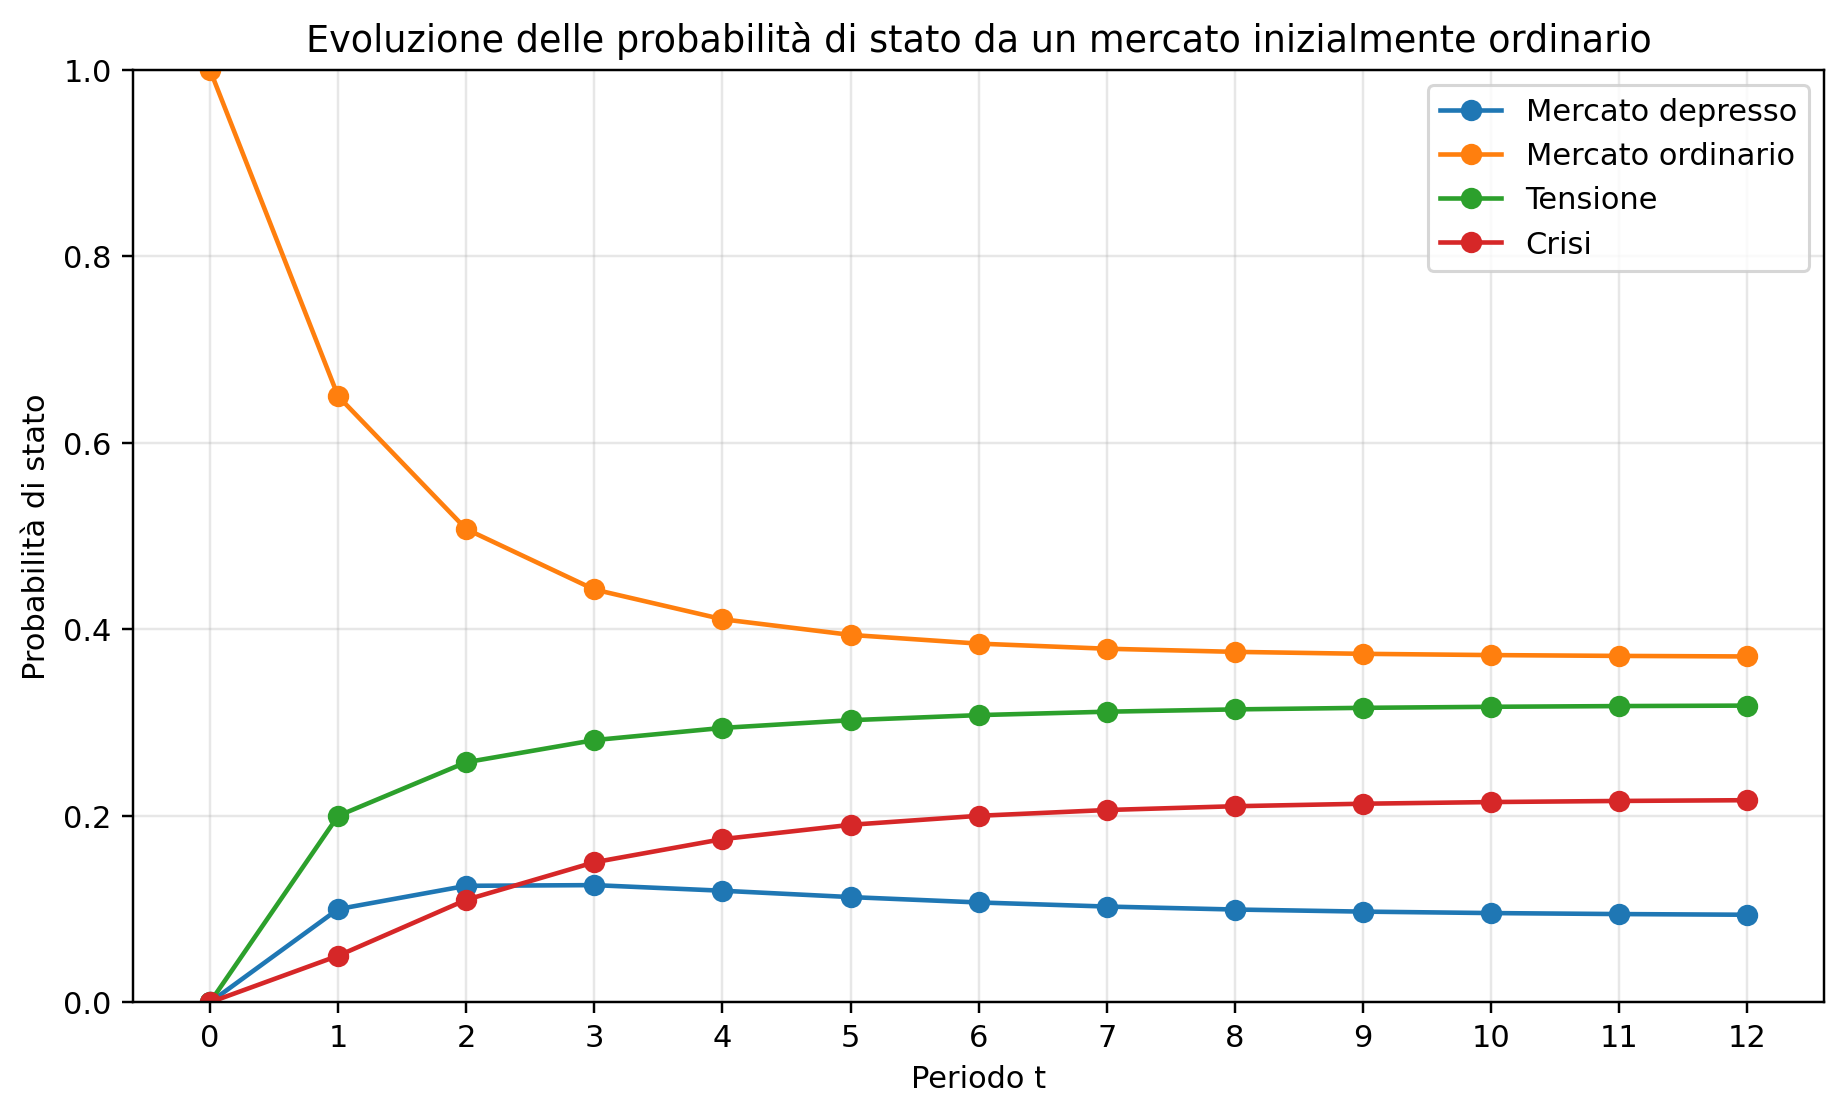
\includegraphics[width=0.60\textwidth]{../graphics/Cap08_Evoluzione_probabilita_stato.png}
\end{center}

\medskip

\begin{center}
\alert{\small Queste sono le probabilit\`{a} di \emph{occupare} lo
stato di crisi alla data considerata, non di entrarvi per la prima
volta.}
\end{center}

%TCIMACRO{\TeXButton{Transition: Box Out}{\transboxout}}%
%BeginExpansion
\transboxout%
%EndExpansion
%TCIMACRO{\TeXButton{EndFrame}{\end{frame}}}%
%BeginExpansion
\end{frame}%
%EndExpansion

%***********************************************************
\section{Esercizio in aula}

\subsection{Esercizio A: consegna}

%TCIMACRO{\TeXButton{BeginFrame}{\begin{frame}}}%
%BeginExpansion
\begin{frame}%
%EndExpansion

\QTR{frametitle}{Esercizio A: il mercato parte dalla tensione}

Si consideri la matrice $P$ dei regimi del mercato elettrico. Il
mercato si trova inizialmente nello stato di \textbf{tensione}. Si
utilizzi la matrice

\[
P^2
=
\begin{pmatrix}
0.3900 & 0.4000 & 0.1700 & 0.0400\\
0.1250 & 0.5075 & 0.2575 & 0.1100\\
0.0250 & 0.3125 & 0.3875 & 0.2750\\
0.0100 & 0.2075 & 0.3875 & 0.3950
\end{pmatrix}.
\]

\medskip

\begin{enumerate}
\item[1.] Costruire la distribuzione iniziale $\pi_{0}$.

\item[2.] Calcolare la distribuzione degli stati dopo due periodi.

\item[3.] Determinare la probabilit\`{a} che il mercato sia in
condizioni ordinarie o depresse dopo due periodi.

\item[4.] Confrontare tale probabilit\`{a} con la probabilit\`{a} di
trovarsi in tensione o in crisi.
\end{enumerate}

\medskip

\begin{center}
{\small Lavoro individuale o a coppie: circa 9 minuti. Seguir\`{a} la
discussione.}
\end{center}

%TCIMACRO{\TeXButton{Transition: Box Out}{\transboxout}}%
%BeginExpansion
\transboxout%
%EndExpansion
%TCIMACRO{\TeXButton{EndFrame}{\end{frame}}}%
%BeginExpansion
\end{frame}%
%EndExpansion

%***********************************************************
\subsection{Esercizio A: discussione}

%TCIMACRO{\TeXButton{BeginFrame}{\begin{frame}}}%
%BeginExpansion
\begin{frame}%
%EndExpansion

\QTR{frametitle}{Esercizio A: discussione}

%TCIMACRO{\TeXButton{Transparency}{\setbeamercovered{transparent=20}}}%
%BeginExpansion
\setbeamercovered{transparent=20}%
%EndExpansion

Raccogliamo e verifichiamo i risultati.

\medskip

\begin{stepitemize}
\item Quale riga di $P^2$ avete utilizzato, e perch\'{e}?

\item Partendo dalla tensione, \`{e} pi\`{u} probabile che dopo due
periodi il mercato sia rientrato (ordinario o depresso) oppure che si
trovi ancora in tensione o in crisi?
\end{stepitemize}

\medskip

Domanda di interpretazione:

\begin{stepitemize}
\item Perch\'{e} questo risultato \textbf{non} pu\`{o} essere
interpretato come previsione empirica per il periodo successivo a uno
shock strutturale, senza verificare l'omogeneit\`{a} temporale?
\end{stepitemize}

\medskip

\begin{center}
{\small Richiamo: la propriet\`{a} di Markov riguarda l'informazione
necessaria; l'omogeneit\`{a} riguarda la stabilit\`{a} nel tempo del
meccanismo di transizione. Il calcolo usa \emph{entrambe}.}
\end{center}

%TCIMACRO{\TeXButton{Transition: Box Out}{\transboxout}}%
%BeginExpansion
\transboxout%
%EndExpansion
%TCIMACRO{\TeXButton{EndFrame}{\end{frame}}}%
%BeginExpansion
\end{frame}%
%EndExpansion

%***********************************************************
\section{Struttura dello spazio degli stati}

\subsection{Accessibilit\`{a} e comunicazione}

%TCIMACRO{\TeXButton{BeginFrame}{\begin{frame}}}%
%BeginExpansion
\begin{frame}%
%EndExpansion

\QTR{frametitle}{Accessibilit\`{a} e comunicazione tra stati}

%TCIMACRO{\TeXButton{Transparency}{\setbeamercovered{transparent=20}}}%
%BeginExpansion
\setbeamercovered{transparent=20}%
%EndExpansion

La matrice $P$ determina anche la \textbf{struttura dei collegamenti}
tra gli stati.

\medskip

\begin{stepitemize}
\item Lo stato $j$ \`{e} \textbf{accessibile} da $i$ se esiste
$n\geq 0$ tale che $p_{ij}^{(n)}>0$. Si scrive $i\rightsquigarrow j$.
Non serve un passaggio diretto: basta un percorso di stati intermedi
con transizioni di probabilit\`{a} positiva. Per convenzione $P^{0}=I$,
quindi ogni stato \`{e} accessibile da se stesso.

\item Gli stati $i$ e $j$ \textbf{comunicano} se ciascuno \`{e}
accessibile dall'altro: $i\rightsquigarrow j$ e $j\rightsquigarrow i$.
Si scrive $i\leftrightarrow j$.

\item La comunicazione \`{e} una relazione di equivalenza: suddivide
lo spazio degli stati in insiemi disgiunti, le \textbf{classi
comunicanti}.
\end{stepitemize}

\medskip

\begin{center}
{\small Sul grafo: $i\rightsquigarrow j$ se esiste un percorso
orientato da $i$ a $j$; $i\leftrightarrow j$ se esistono percorsi in
entrambe le direzioni.}
\end{center}

%TCIMACRO{\TeXButton{Transition: Box Out}{\transboxout}}%
%BeginExpansion
\transboxout%
%EndExpansion
%TCIMACRO{\TeXButton{EndFrame}{\end{frame}}}%
%BeginExpansion
\end{frame}%
%EndExpansion

%***********************************************************
\subsection{Insiemi chiusi e stati assorbenti}

%TCIMACRO{\TeXButton{BeginFrame}{\begin{frame}}}%
%BeginExpansion
\begin{frame}%
%EndExpansion

\QTR{frametitle}{Insiemi chiusi e stati assorbenti}

%TCIMACRO{\TeXButton{Transparency}{\setbeamercovered{transparent=20}}}%
%BeginExpansion
\setbeamercovered{transparent=20}%
%EndExpansion

Un sottoinsieme non vuoto $C\subseteq\mathcal{I}$ si dice
\textbf{chiuso} se la catena non pu\`{o} uscirne:

\[
p_{ij}=0
\qquad
\text{per ogni }i\in C
\text{ e ogni }j\notin C.
\]

Se la catena entra in un insieme chiuso, tutti gli stati successivi
appartengono allo stesso insieme.

\medskip

Caso particolare: lo stato $i$ \`{e} \textbf{assorbente} se

\[
p_{ii}=1.
\]

\medskip

\begin{stepitemize}
\item Se $i$ \`{e} assorbente, allora $p_{ij}=0$ per ogni $j\neq i$;

\item l'insieme $\{i\}$ costituisce, da solo, una classe chiusa.
\end{stepitemize}

%TCIMACRO{\TeXButton{Transition: Box Out}{\transboxout}}%
%BeginExpansion
\transboxout%
%EndExpansion
%TCIMACRO{\TeXButton{EndFrame}{\end{frame}}}%
%BeginExpansion
\end{frame}%
%EndExpansion

%***********************************************************
\subsection{La catena di migrazione del rating}

%TCIMACRO{\TeXButton{BeginFrame}{\begin{frame}}}%
%BeginExpansion
\begin{frame}%
%EndExpansion

\QTR{frametitle}{Esempio: migrazione del rating con default}

%TCIMACRO{\TeXButton{Transparency}{\setbeamercovered{transparent=20}}}%
%BeginExpansion
\setbeamercovered{transparent=20}%
%EndExpansion

Stati:
$\mathcal{I}
=
\{
1=\text{alta qualit\`{a}},
\,
2=\text{qualit\`{a} intermedia},
\,
3=\text{speculative grade},
\,
4=\text{default}
\}$.

\medskip

Matrice di transizione annuale stilizzata:

\[
P_R
=
\begin{pmatrix}
0.80 & 0.18 & 0.02 & 0.00\\
0.08 & 0.75 & 0.14 & 0.03\\
0.02 & 0.18 & 0.65 & 0.15\\
0.00 & 0.00 & 0.00 & 1.00
\end{pmatrix}
\]

\medskip

\begin{stepitemize}
\item Gli stati $1$, $2$ e $3$ comunicano tra loro: un emittente
pu\`{o} migliorare o peggiorare il proprio merito creditizio.

\item Lo stato $4$ \`{e} \textbf{assorbente}: $p_{44}=1$. Dal default
non si ritorna nelle altre classi.

\item $\{1,2,3\}$ \`{e} una classe comunicante \textbf{non chiusa};
$\{4\}$ \`{e} una classe comunicante \textbf{chiusa}.
\end{stepitemize}

%TCIMACRO{\TeXButton{Transition: Box Out}{\transboxout}}%
%BeginExpansion
\transboxout%
%EndExpansion
%TCIMACRO{\TeXButton{EndFrame}{\end{frame}}}%
%BeginExpansion
\end{frame}%
%EndExpansion

%***********************************************************
\subsection{Grafo della catena di rating}

%TCIMACRO{\TeXButton{BeginFrame}{\begin{frame}}}%
%BeginExpansion
\begin{frame}%
%EndExpansion

\QTR{frametitle}{Grafo della catena di migrazione del rating}

\begin{center}
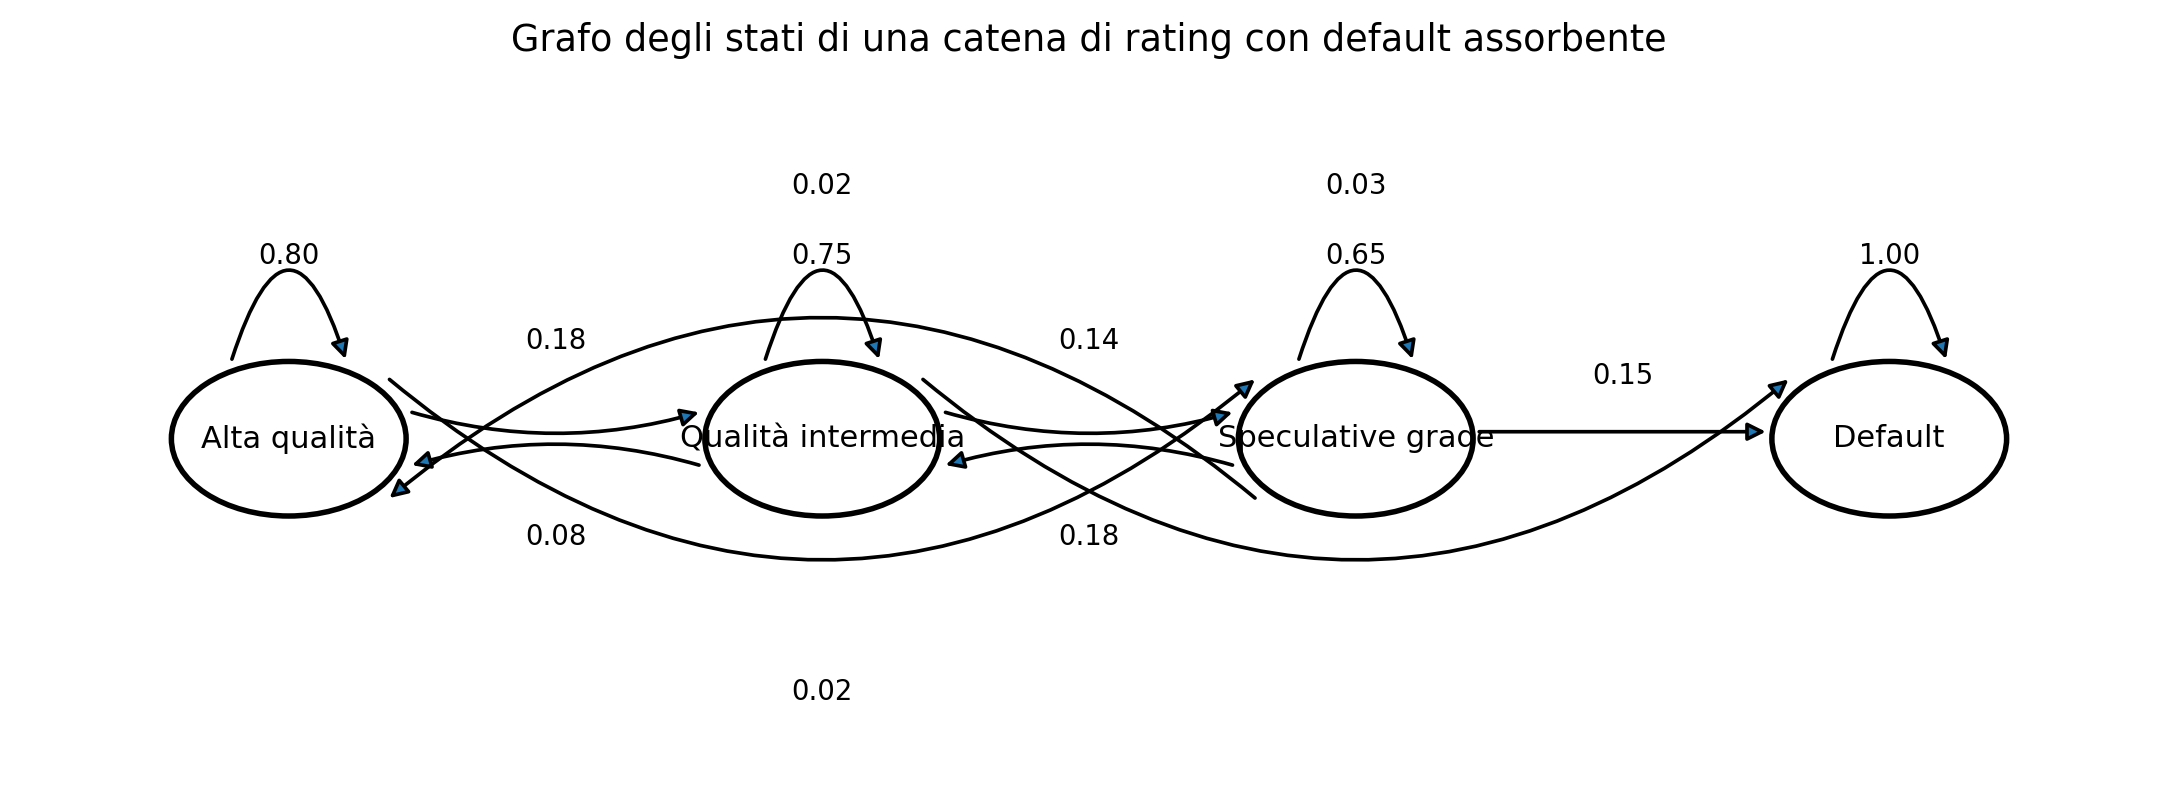
\includegraphics[width=0.90\textwidth]{../graphics/Cap08_Grafo_rating_default.png}
\end{center}

\medskip

\begin{center}
{\small Gli stati non in default comunicano tra loro, ma possono
condurre alla classe chiusa costituita dal default assorbente.}
\end{center}

%TCIMACRO{\TeXButton{Transition: Box Out}{\transboxout}}%
%BeginExpansion
\transboxout%
%EndExpansion
%TCIMACRO{\TeXButton{EndFrame}{\end{frame}}}%
%BeginExpansion
\end{frame}%
%EndExpansion

%***********************************************************
\subsection{Stati transitori e ricorrenti}

%TCIMACRO{\TeXButton{BeginFrame}{\begin{frame}}}%
%BeginExpansion
\begin{frame}%
%EndExpansion

\QTR{frametitle}{Stati transitori e stati ricorrenti}

%TCIMACRO{\TeXButton{Transparency}{\setbeamercovered{transparent=20}}}%
%BeginExpansion
\setbeamercovered{transparent=20}%
%EndExpansion

La classificazione riguarda la possibilit\`{a} di \textbf{ritornare}
nello stato di partenza.

\medskip

\begin{stepitemize}
\item Uno stato $i$ \`{e} \textbf{ricorrente} se, partendo da $i$, la
probabilit\`{a} di ritornarvi prima o poi \`{e} pari a uno.

\item Uno stato $i$ \`{e} \textbf{transitorio} se tale probabilit\`{a}
\`{e} minore di uno.
\end{stepitemize}

\medskip

Per una catena \textbf{finita} valgono tre risultati:

\begin{stepitemize}
\item gli stati di una classe comunicante \textbf{chiusa} sono
ricorrenti;

\item gli stati di una classe comunicante \textbf{non chiusa} sono
transitori;

\item almeno una classe comunicante chiusa deve esistere.
\end{stepitemize}

\medskip

\begin{center}
{\small Nella catena di rating: $1$, $2$ e $3$ sono transitori (si
pu\`{o} uscire dalla loro classe entrando nel default); $4$ \`{e}
ricorrente e assorbente.}
\end{center}

%TCIMACRO{\TeXButton{Transition: Box Out}{\transboxout}}%
%BeginExpansion
\transboxout%
%EndExpansion
%TCIMACRO{\TeXButton{EndFrame}{\end{frame}}}%
%BeginExpansion
\end{frame}%
%EndExpansion

%***********************************************************
\subsection{Irriducibilit\`{a} e aperiodicit\`{a}}

%TCIMACRO{\TeXButton{BeginFrame}{\begin{frame}}}%
%BeginExpansion
\begin{frame}%
%EndExpansion

\QTR{frametitle}{Irriducibilit\`{a} e aperiodicit\`{a}}

%TCIMACRO{\TeXButton{Transparency}{\setbeamercovered{transparent=20}}}%
%BeginExpansion
\setbeamercovered{transparent=20}%
%EndExpansion

Una catena \`{e} \textbf{irriducibile} se tutti gli stati comunicano
tra loro: $\mathcal{I}$ costituisce un'unica classe comunicante. Una
catena finita irriducibile non possiede stati transitori.

\medskip

\begin{stepitemize}
\item La catena dei regimi del mercato elettrico \`{e}
\textbf{irriducibile}: $p_{41}=0$, ma il percorso
\[
\text{crisi}
\longrightarrow
\text{ordinario}
\longrightarrow
\text{depresso}
\]
ha probabilit\`{a} positiva, quindi $4\rightsquigarrow 1$.

\item La catena di rating \`{e} \textbf{riducibile}: il default non
comunica con gli stati non in default.
\end{stepitemize}

\medskip

Condizione sufficiente di \textbf{aperiodicit\`{a}}: se $p_{ii}>0$, un
ritorno \`{e} possibile dopo un solo periodo e lo stato $i$ \`{e}
aperiodico (trattazione completa della periodicit\`{a}: slide di
back-up e manuale).

\medskip

\begin{center}
{\small Nel mercato elettrico $p_{ii}>0$ per ogni $i$: catena finita,
irriducibile e aperiodica. Queste propriet\`{a} saranno decisive per la
distribuzione stazionaria.}
\end{center}

%TCIMACRO{\TeXButton{Transition: Box Out}{\transboxout}}%
%BeginExpansion
\transboxout%
%EndExpansion
%TCIMACRO{\TeXButton{EndFrame}{\end{frame}}}%
%BeginExpansion
\end{frame}%
%EndExpansion

%***********************************************************
\section{Distribuzioni stazionarie e lungo periodo}

\subsection{Definizione}

%TCIMACRO{\TeXButton{BeginFrame}{\begin{frame}}}%
%BeginExpansion
\begin{frame}%
%EndExpansion

\QTR{frametitle}{Distribuzione stazionaria}

%TCIMACRO{\TeXButton{Transparency}{\setbeamercovered{transparent=20}}}%
%BeginExpansion
\setbeamercovered{transparent=20}%
%EndExpansion

Al crescere dell'orizzonte, la distribuzione $\pi_{t}=\pi_{0}P^{t}$
tende a stabilizzarsi? Esiste una distribuzione che resta invariata
sotto l'azione di $P$?

\medskip

Una distribuzione di probabilit\`{a}
$\pi=
\begin{pmatrix}
\pi_{1} & \cdots & \pi_{m}
\end{pmatrix}$
si dice \textbf{stazionaria} per $P$ se

\[
\pi=\pi P,
\qquad
\pi_{i}\geq 0,
\qquad
\sum_{i=1}^{m}\pi_{i}=1.
\]

\medskip

\begin{stepitemize}
\item Se la distribuzione iniziale coincide con una distribuzione
stazionaria, $\pi_{0}=\pi$, allora
\[
\pi_{t}=\pi P^{t}=\pi
\qquad
\text{per ogni }t\geq 0.
\]

\item La \textbf{distribuzione} degli stati resta invariata nel tempo,
anche se la catena \textbf{continua a transitare} casualmente tra gli
stati.
\end{stepitemize}

%TCIMACRO{\TeXButton{Transition: Box Out}{\transboxout}}%
%BeginExpansion
\transboxout%
%EndExpansion
%TCIMACRO{\TeXButton{EndFrame}{\end{frame}}}%
%BeginExpansion
\end{frame}%
%EndExpansion

%***********************************************************
\subsection{Calcolo della distribuzione stazionaria}

%TCIMACRO{\TeXButton{BeginFrame}{\begin{frame}}}%
%BeginExpansion
\begin{frame}%
%EndExpansion

\QTR{frametitle}{Calcolo: il caso del mercato elettrico}

%TCIMACRO{\TeXButton{Transparency}{\setbeamercovered{transparent=20}}}%
%BeginExpansion
\setbeamercovered{transparent=20}%
%EndExpansion

Si risolve il sistema $\pi=\pi P$ con il vincolo
$\sum_{i=1}^{m}\pi_{i}=1$. Per la matrice $P$ dei regimi del mercato
elettrico:

\[
\begin{cases}
\pi_{1}
=
0.60\pi_{1}+0.10\pi_{2},\\
\pi_{2}
=
0.30\pi_{1}+0.65\pi_{2}+0.25\pi_{3}+0.10\pi_{4},\\
\pi_{3}
=
0.10\pi_{1}+0.20\pi_{2}+0.50\pi_{3}+0.35\pi_{4},\\
\pi_{4}
=
0.05\pi_{2}+0.25\pi_{3}+0.55\pi_{4},\\
\pi_{1}+\pi_{2}+\pi_{3}+\pi_{4}=1.
\end{cases}
\]

Le equazioni di $\pi=\pi P$ non sono tutte indipendenti (le righe di
$P$ sommano a uno): una \`{e} ridondante e viene sostituita dal vincolo
di normalizzazione. La soluzione \`{e}

\[
\pi
=
\begin{pmatrix}
\dfrac{11}{119}
&
\dfrac{44}{119}
&
\dfrac{38}{119}
&
\dfrac{26}{119}
\end{pmatrix}
\approx
\begin{pmatrix}
0.0924 & 0.3697 & 0.3193 & 0.2185
\end{pmatrix}.
\]

\medskip

\begin{center}
{\small Verifica diretta: $\pi P=\pi$, componenti non negative e a
somma uno.}
\end{center}

%TCIMACRO{\TeXButton{Transition: Box Out}{\transboxout}}%
%BeginExpansion
\transboxout%
%EndExpansion
%TCIMACRO{\TeXButton{EndFrame}{\end{frame}}}%
%BeginExpansion
\end{frame}%
%EndExpansion

%***********************************************************
\subsection{Esistenza, unicit\`{a} e convergenza}

%TCIMACRO{\TeXButton{BeginFrame}{\begin{frame}}}%
%BeginExpansion
\begin{frame}%
%EndExpansion

\QTR{frametitle}{Tre risultati distinti}

%TCIMACRO{\TeXButton{Transparency}{\setbeamercovered{transparent=20}}}%
%BeginExpansion
\setbeamercovered{transparent=20}%
%EndExpansion

\begin{stepenumerate}
\item[1.] \textbf{Esistenza.} Ogni catena di Markov con spazio degli
stati finito possiede almeno una distribuzione stazionaria.

\item[2.] \textbf{Unicit\`{a}.} Una catena finita e
\textbf{irriducibile} possiede un'unica distribuzione stazionaria
$\pi$, con $\pi_{i}>0$ per ogni $i\in\mathcal{I}$.

\item[3.] \textbf{Convergenza.} Se la catena finita \`{e} irriducibile
e \textbf{aperiodica}, allora, per ogni distribuzione iniziale
$\pi_{0}$,
\[
\pi_{0}P^{t}\longrightarrow\pi
\qquad
\text{per }t\longrightarrow\infty.
\]
Tutte le righe di $P^{t}$ convergono alla stessa distribuzione $\pi$:
l'effetto dello stato iniziale si attenua progressivamente.
\end{stepenumerate}

\medskip

\begin{stepitemize}
\item Una catena riducibile pu\`{o} avere pi\`{u} distribuzioni
stazionarie.

\item Una catena irriducibile ma \textbf{periodica} ha $\pi$ unica, ma
$\pi_{0}P^{t}$ pu\`{o} continuare a oscillare senza convergere.
\end{stepitemize}

%TCIMACRO{\TeXButton{Transition: Box Out}{\transboxout}}%
%BeginExpansion
\transboxout%
%EndExpansion
%TCIMACRO{\TeXButton{EndFrame}{\end{frame}}}%
%BeginExpansion
\end{frame}%
%EndExpansion

%***********************************************************
\subsection{Convergenza: il caso del mercato elettrico}

%TCIMACRO{\TeXButton{BeginFrame}{\begin{frame}}}%
%BeginExpansion
\begin{frame}%
%EndExpansion

\QTR{frametitle}{Convergenza alla distribuzione stazionaria}

La catena dei regimi del mercato elettrico \`{e} finita, irriducibile e
aperiodica: per ogni $\pi_{0}$,

\[
\pi_{0}P^{t}
\longrightarrow
\begin{pmatrix}
0.0924 & 0.3697 & 0.3193 & 0.2185
\end{pmatrix}.
\]

\begin{center}
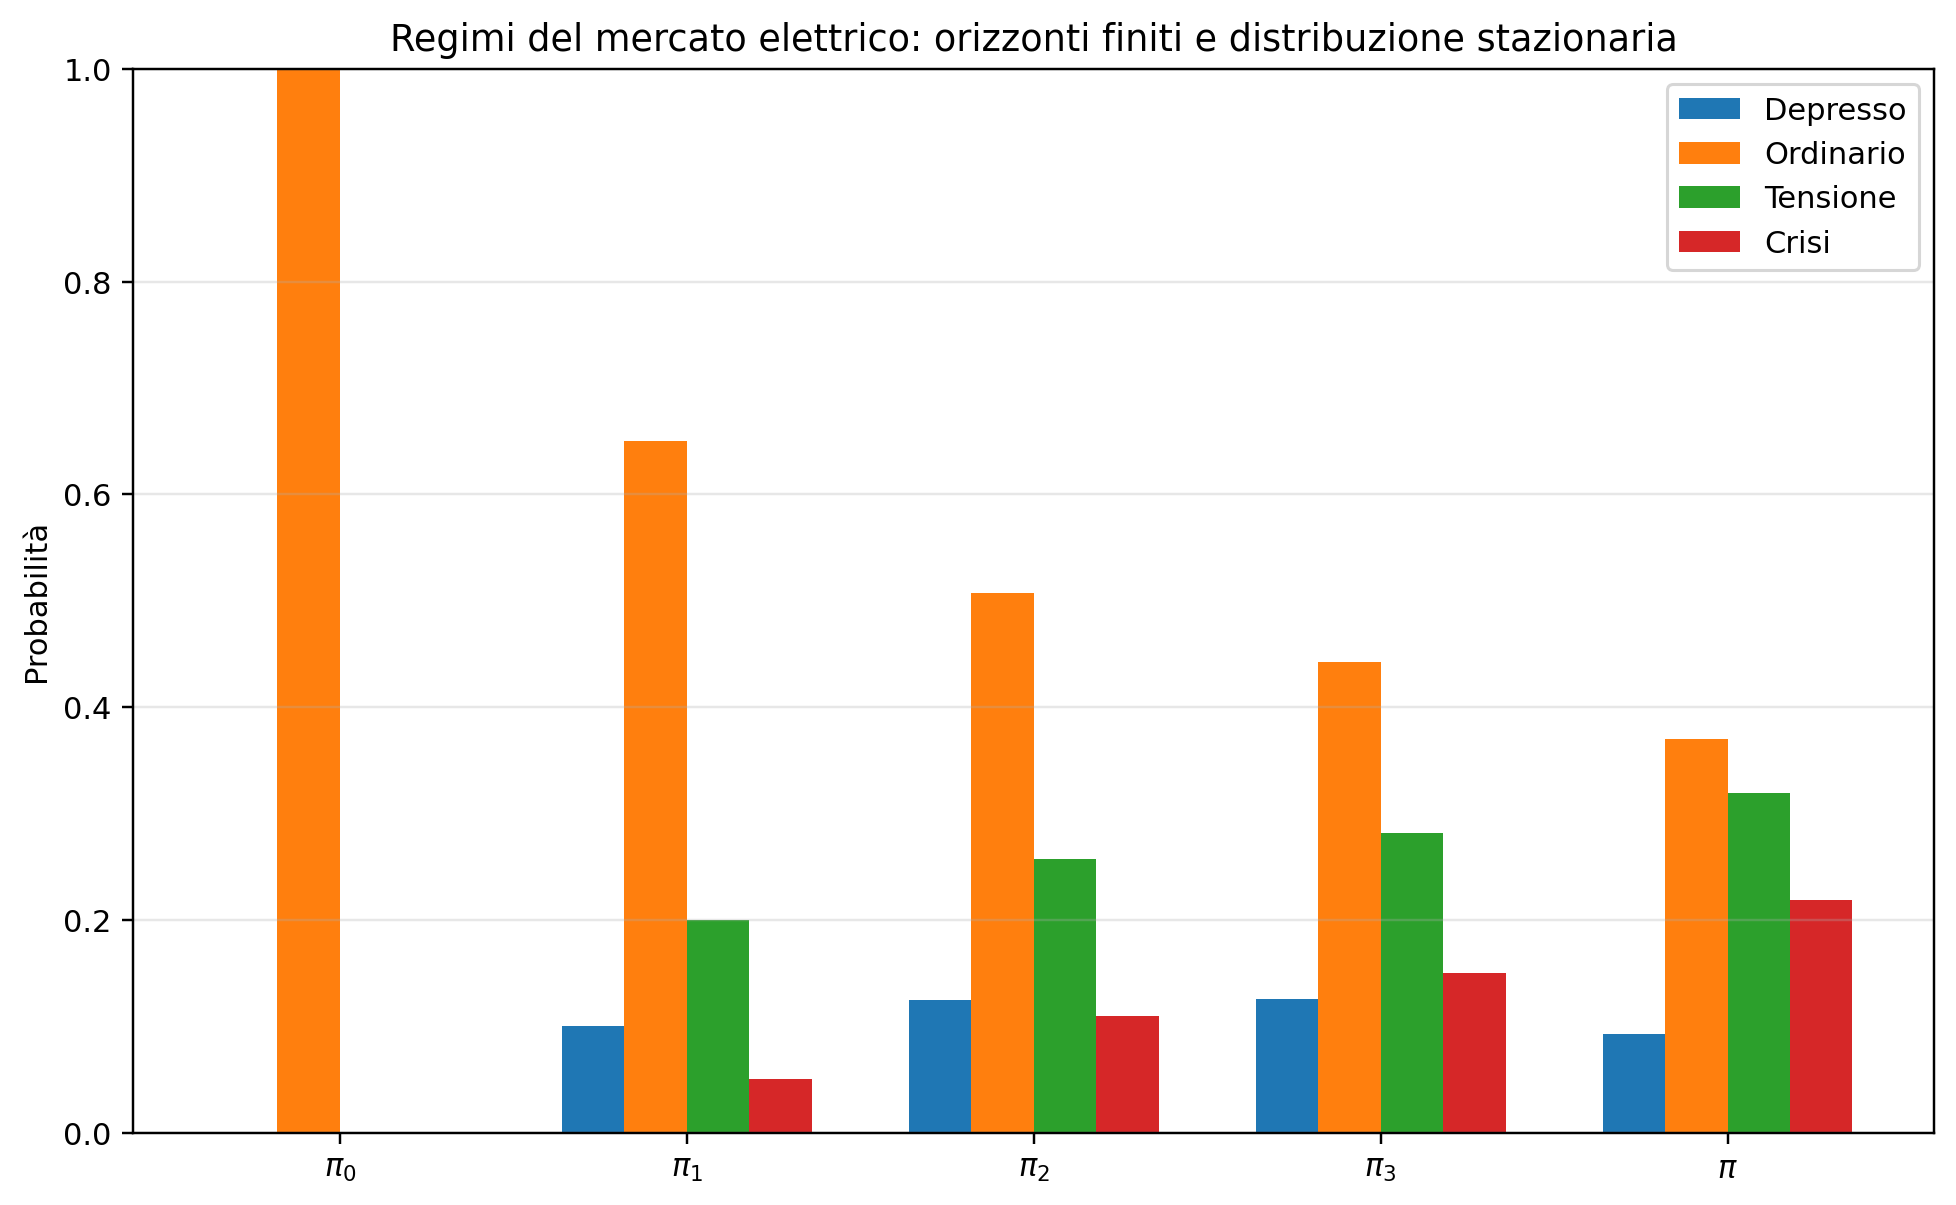
\includegraphics[width=0.72\textwidth]{../graphics/Cap08_Orizzonti_distribuzione_stazionaria.png}
\end{center}

\medskip

\begin{center}
{\small Partendo dallo stato $2$ (ordinario), la massa di
probabilit\`{a} si redistribuisce e tende alla distribuzione di lungo
periodo.}
\end{center}

%TCIMACRO{\TeXButton{Transition: Box Out}{\transboxout}}%
%BeginExpansion
\transboxout%
%EndExpansion
%TCIMACRO{\TeXButton{EndFrame}{\end{frame}}}%
%BeginExpansion
\end{frame}%
%EndExpansion

%***********************************************************
\subsection{Interpretazione economica e limiti}

%TCIMACRO{\TeXButton{BeginFrame}{\begin{frame}}}%
%BeginExpansion
\begin{frame}%
%EndExpansion

\QTR{frametitle}{Interpretazione economica e limiti}

%TCIMACRO{\TeXButton{Transparency}{\setbeamercovered{transparent=20}}}%
%BeginExpansion
\setbeamercovered{transparent=20}%
%EndExpansion

Per una catena finita irriducibile, $\pi_{i}$ \`{e} interpretabile come
\textbf{quota di lungo periodo} trascorsa nello stato $i$: indicando
con $N_{i}(T)$ il numero di periodi trascorsi in $i$ fino al tempo
$T$,

\[
\frac{N_{i}(T)}{T+1}
\longrightarrow
\pi_{i}.
\]

Nel caso guida, $\pi_{4}\approx 0.2185$: quota teorica di lungo periodo
trascorsa nello stato $4$ (crisi).

\medskip

\begin{stepitemize}
\item La distribuzione stazionaria \`{e} condizionata alla matrice
adottata: $P\longrightarrow\pi$. Se cambiano regolazione, struttura
produttiva o comportamenti, pu\`{o} cambiare $P$ e quindi $\pi$.

\item Esempio: una matrice stimata prima della Market Stability
Reserve pu\`{o} generare una $\pi$ diversa da quella successiva alla
riforma.

\item La stazionariet\`{a} \textbf{non} implica che il sistema
economico sia strutturalmente immutabile, e $\pi$ non va interpretata
automaticamente come equilibrio economico.
\end{stepitemize}

%TCIMACRO{\TeXButton{Transition: Box Out}{\transboxout}}%
%BeginExpansion
\transboxout%
%EndExpansion
%TCIMACRO{\TeXButton{EndFrame}{\end{frame}}}%
%BeginExpansion
\end{frame}%
%EndExpansion

%***********************************************************
\section{Esercizio in aula: rating e default}

\subsection{Esercizio B: consegna}

%TCIMACRO{\TeXButton{BeginFrame}{\begin{frame}}}%
%BeginExpansion
\begin{frame}%
%EndExpansion

\QTR{frametitle}{Esercizio B: emittente speculative grade}

%TCIMACRO{\TeXButton{Transparency}{\setbeamercovered{transparent=20}}}%
%BeginExpansion
\setbeamercovered{transparent=20}%
%EndExpansion

Un emittente ha oggi rating \textbf{speculative grade} (stato $3$).
Si utilizzino la matrice $P_R$ e le potenze

{\small
\[
P_R^2
=
\begin{pmatrix}
0.655 & 0.283 & 0.054 & 0.008\\
0.127 & 0.602 & 0.198 & 0.073\\
0.043 & 0.256 & 0.448 & 0.253\\
0.000 & 0.000 & 0.000 & 1.000
\end{pmatrix}
,
P_R^3
=
\begin{pmatrix}
0.539 & 0.321 & 0.082 & 0.058\\
0.154 & 0.510 & 0.215 & 0.121\\
0.064 & 0.280 & 0.328 & 0.328\\
0.000 & 0.000 & 0.000 & 1.000
\end{pmatrix}
\]
}

\medskip

\begin{enumerate}
\item[1.] Costruire la distribuzione iniziale $\pi_{0}$.

\item[2.] Determinare la distribuzione del rating dopo tre anni e la
probabilit\`{a} di default entro uno, due e tre anni.

\item[3.] Verificare che
$\pi_{D}=
\begin{pmatrix}
0 & 0 & 0 & 1
\end{pmatrix}$
\`{e} una distribuzione stazionaria per $P_R$.

\item[4.] Con il grafo della catena: perch\'{e} da ogni stato non in
default il default \`{e} accessibile, mentre non vale il viceversa?
\end{enumerate}

\medskip

\begin{center}
{\small Lavoro individuale o a coppie: circa 9 minuti. Seguir\`{a} la
discussione.}
\end{center}

%TCIMACRO{\TeXButton{Transition: Box Out}{\transboxout}}%
%BeginExpansion
\transboxout%
%EndExpansion
%TCIMACRO{\TeXButton{EndFrame}{\end{frame}}}%
%BeginExpansion
\end{frame}%
%EndExpansion

%***********************************************************
\subsection{Esercizio B: discussione}

%TCIMACRO{\TeXButton{BeginFrame}{\begin{frame}}}%
%BeginExpansion
\begin{frame}%
%EndExpansion

\QTR{frametitle}{Esercizio B: discussione}

%TCIMACRO{\TeXButton{Transparency}{\setbeamercovered{transparent=20}}}%
%BeginExpansion
\setbeamercovered{transparent=20}%
%EndExpansion

Raccogliamo e verifichiamo i risultati.

\medskip

\begin{stepitemize}
\item Nella slide sull'evoluzione dal mercato ordinario avevamo
avvertito: probabilit\`{a} di \emph{occupare} lo stato, non di
entrarvi per la prima volta. Perch\'{e} qui, invece, la
probabilit\`{a} di trovarsi in default al terzo anno \textbf{coincide}
con la probabilit\`{a} di default \emph{entro} tre anni?

\item La catena di rating \`{e} riducibile: eppure la distribuzione
stazionaria \`{e} unica. Come si concilia con i risultati visti?

\item $\pi_{D}$ dice che nel lungo periodo tutta la probabilit\`{a} si
concentra nel default. \`{E} una previsione sensata sulla
distribuzione dei rating di un'economia?
\end{stepitemize}

\medskip

\begin{center}
{\small Lo stato assorbente accumula: occupazione ed entrata
coincidono. La conclusione vale per un singolo emittente seguito
indefinitamente, non per il sistema economico: nuovi ingressi,
fusioni, cessazioni e sostituzioni sono fuori dal modello.}
\end{center}

%TCIMACRO{\TeXButton{Transition: Box Out}{\transboxout}}%
%BeginExpansion
\transboxout%
%EndExpansion
%TCIMACRO{\TeXButton{EndFrame}{\end{frame}}}%
%BeginExpansion
\end{frame}%
%EndExpansion

%***********************************************************
\section{Sintesi}

\subsection{Sintesi e raccordo}

%TCIMACRO{\TeXButton{BeginFrame}{\begin{frame}}}%
%BeginExpansion
\begin{frame}%
%EndExpansion

\QTR{frametitle}{Sintesi e raccordo con il Capitolo 9}

%TCIMACRO{\TeXButton{Transparency}{\setbeamercovered{transparent=20}}}%
%BeginExpansion
\setbeamercovered{transparent=20}%
%EndExpansion

Il percorso della lezione:

\[
\text{stati}
\longrightarrow
P
\longrightarrow
P^{n}
\longrightarrow
\pi_{t}=\pi_{0}P^{t}
\longrightarrow
\text{struttura}
\longrightarrow
\pi=\pi P.
\]

\medskip

Tre avvertenze da portare con s\'{e}:

\begin{stepitemize}
\item la propriet\`{a} di \textbf{Markov} e l'\textbf{omogeneit\`{a}}
temporale sono ipotesi distinte, ed entrambe vanno giustificate nel
caso applicativo;

\item $\pi_{t}(i)$ \`{e} la probabilit\`{a} di \emph{occupare} lo stato
$i$ al tempo $t$; coincide con la probabilit\`{a} di esservi entrati
solo in casi particolari, come lo stato assorbente;

\item la distribuzione stazionaria \`{e} condizionata alla matrice
adottata ($P\longrightarrow\pi$) e non va interpretata automaticamente
come equilibrio economico.
\end{stepitemize}

\medskip

\begin{center}
{\small Nel Capitolo 9, agli stati verranno associate esposizioni e
perdite: dalle probabilit\`{a} di transizione alle misure di rischio
$\VaR$ e $\CVaR$.}
\end{center}

%TCIMACRO{\TeXButton{Transition: Box Out}{\transboxout}}%
%BeginExpansion
\transboxout%
%EndExpansion
%TCIMACRO{\TeXButton{EndFrame}{\end{frame}}}%
%BeginExpansion
\end{frame}%
%EndExpansion

%***********************************************************
\section{Sintesi}

\subsection{Sintesi e raccordo}

%TCIMACRO{\TeXButton{BeginFrame}{\begin{frame}}}%
%BeginExpansion
\begin{frame}%
%EndExpansion

\QTR{frametitle}{Sintesi e raccordo con il Capitolo 9}

%TCIMACRO{\TeXButton{Transparency}{\setbeamercovered{transparent=20}}}%
%BeginExpansion
\setbeamercovered{transparent=20}%
%EndExpansion

Il percorso della lezione:

\[
\text{stati}
\longrightarrow
P
\longrightarrow
P^{n}
\longrightarrow
\pi_{t}=\pi_{0}P^{t}
\longrightarrow
\text{struttura}
\longrightarrow
\pi=\pi P.
\]

\medskip

Tre avvertenze da portare con s\'{e}:

\begin{stepitemize}
\item la propriet\`{a} di \textbf{Markov} e l'\textbf{omogeneit\`{a}}
temporale sono ipotesi distinte, ed entrambe vanno giustificate nel
caso applicativo;

\item $\pi_{t}(i)$ \`{e} la probabilit\`{a} di \emph{occupare} lo stato
$i$ al tempo $t$; coincide con la probabilit\`{a} di esservi entrati
solo in casi particolari, come lo stato assorbente;

\item la distribuzione stazionaria \`{e} condizionata alla matrice
adottata ($P\longrightarrow\pi$) e non va interpretata automaticamente
come equilibrio economico.
\end{stepitemize}

\medskip

\begin{center}
{\small Nel Capitolo 9, agli stati verranno associate esposizioni e
perdite: dalle probabilit\`{a} di transizione alle misure di rischio
$\VaR$ e $\CVaR$.}
\end{center}

%TCIMACRO{\TeXButton{Transition: Box Out}{\transboxout}}%
%BeginExpansion
\transboxout%
%EndExpansion
%TCIMACRO{\TeXButton{EndFrame}{\end{frame}}}%
%BeginExpansion
\end{frame}%
%EndExpansion

%***********************************************************
\section{Back-up ed esercizi}

\subsection{Back-up: periodicit\`{a}}

%TCIMACRO{\TeXButton{BeginFrame}{\begin{frame}}}%
%BeginExpansion
\begin{frame}%
%EndExpansion

\QTR{frametitle}{Back-up: periodicit\`{a} di uno stato}

%TCIMACRO{\TeXButton{Transparency}{\setbeamercovered{transparent=20}}}%
%BeginExpansion
\setbeamercovered{transparent=20}%
%EndExpansion

Il \textbf{periodo} dello stato $i$ \`{e}

\[
d(i)
=
\gcd
\{
n\geq 1
:
p_{ii}^{(n)}>0
\},
\]

il massimo comune divisore delle lunghezze dei possibili ritorni in
$i$. Lo stato \`{e} \textbf{aperiodico} se $d(i)=1$, \textbf{periodico}
se $d(i)>1$.

\medskip

Esempio di catena ciclica a tre stati:

\[
P_{\mathrm{c}}
=
\begin{pmatrix}
0 & 1 & 0\\
0 & 0 & 1\\
1 & 0 & 0
\end{pmatrix}
\]

\medskip

\begin{stepitemize}
\item Ogni ritorno allo stato di partenza richiede un multiplo di $3$
passi: $d(i)=3$ per ogni stato.

\item La condizione $p_{ii}>0$ \`{e} \textbf{sufficiente} ma non
necessaria per l'aperiodicit\`{a}.
\end{stepitemize}

%TCIMACRO{\TeXButton{Transition: Box Out}{\transboxout}}%
%BeginExpansion
\transboxout%
%EndExpansion
%TCIMACRO{\TeXButton{EndFrame}{\end{frame}}}%
%BeginExpansion
\end{frame}%
%EndExpansion

%***********************************************************
\subsection{Back-up: catena periodica e oscillazione}

%TCIMACRO{\TeXButton{BeginFrame}{\begin{frame}}}%
%BeginExpansion
\begin{frame}%
%EndExpansion

\QTR{frametitle}{Back-up: catena periodica, distribuzione che oscilla}

Per $P_{\mathrm{c}}$, partendo dallo stato $1$, la distribuzione
$\pi_{t}$ non converge: la massa di probabilit\`{a} ruota tra gli
stati.

\medskip

\begin{center}
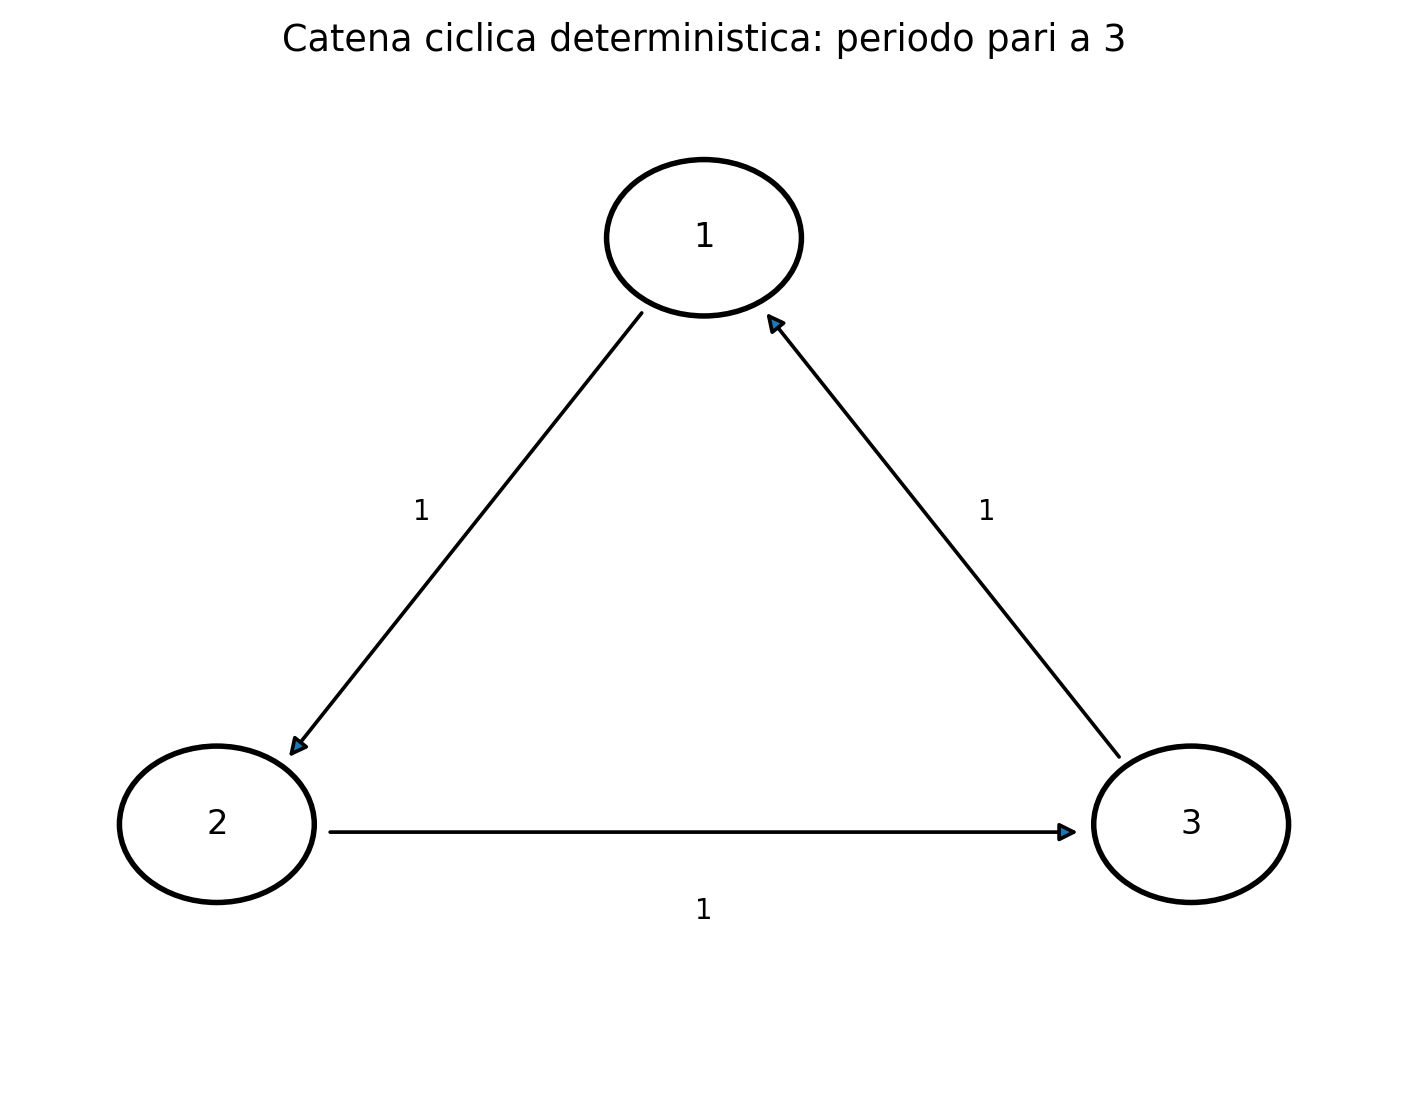
\includegraphics[width=0.68\textwidth]{../graphics/Cap08_Esempio_periodico.png}
\end{center}

\medskip

\begin{center}
{\small La distribuzione stazionaria esiste ed \`{e} unica (catena
irriducibile), ma la convergenza fallisce: manca l'aperiodicit\`{a}.}
\end{center}

%TCIMACRO{\TeXButton{Transition: Box Out}{\transboxout}}%
%BeginExpansion
\transboxout%
%EndExpansion
%TCIMACRO{\TeXButton{EndFrame}{\end{frame}}}%
%BeginExpansion
\end{frame}%
%EndExpansion

%***********************************************************
\subsection{Back-up: caratterizzazione della ricorrenza}

%TCIMACRO{\TeXButton{BeginFrame}{\begin{frame}}}%
%BeginExpansion
\begin{frame}%
%EndExpansion

\QTR{frametitle}{Back-up: ricorrenza e serie dei ritorni}

%TCIMACRO{\TeXButton{Transparency}{\setbeamercovered{transparent=20}}}%
%BeginExpansion
\setbeamercovered{transparent=20}%
%EndExpansion

La classificazione degli stati ammette una caratterizzazione mediante
la serie delle probabilit\`{a} di ritorno:

\begin{stepitemize}
\item lo stato $i$ \`{e} \textbf{ricorrente} se e solo se
\[
\sum_{n=1}^{\infty}p_{ii}^{(n)}=\infty;
\]

\item lo stato $i$ \`{e} \textbf{transitorio} se e solo se
\[
\sum_{n=1}^{\infty}p_{ii}^{(n)}<\infty.
\]
\end{stepitemize}

\medskip

\begin{center}
{\small Intuizione: per uno stato ricorrente i ritorni sono
infinitamente frequenti; per uno stato transitorio le probabilit\`{a}
di ritorno si spengono abbastanza in fretta da rendere la serie
convergente. Dettagli nel manuale.}
\end{center}

%TCIMACRO{\TeXButton{Transition: Box Out}{\transboxout}}%
%BeginExpansion
\transboxout%
%EndExpansion
%TCIMACRO{\TeXButton{EndFrame}{\end{frame}}}%
%BeginExpansion
\end{frame}%
%EndExpansion

%***********************************************************
\subsection{Back-up: esercizio sulle quote di emissione}

%TCIMACRO{\TeXButton{BeginFrame}{\begin{frame}}}%
%BeginExpansion
\begin{frame}%
%EndExpansion

\QTR{frametitle}{Back-up: quote di emissione e cambiamento di regime}

Mercato delle quote di emissione, con matrici stimate prima e dopo una
riforma regolatoria (si vedano i dati dell'esercizio proposto nel
capitolo):

\medskip

\begin{enumerate}
\item[1.] Calcolare la distribuzione stazionaria di
$P_{\mathrm{pre}}$ e quella di $P_{\mathrm{post}}$.

\item[2.] Confrontare le quote di lungo periodo dei diversi regimi di
prezzo nei due casi.

\item[3.] Discutere: che cosa \emph{misura} la differenza tra le due
distribuzioni stazionarie? Quale ipotesi del modello \`{e} venuta meno
nel passaggio dalla prima alla seconda matrice?
\end{enumerate}

\medskip

\begin{center}
{\small \`{E} l'unico esercizio del capitolo che quantifica la rottura
dell'omogeneit\`{a} temporale confrontando due regimi stazionari.}
\end{center}

%TCIMACRO{\TeXButton{Transition: Box Out}{\transboxout}}%
%BeginExpansion
\transboxout%
%EndExpansion
%TCIMACRO{\TeXButton{EndFrame}{\end{frame}}}%
%BeginExpansion
\end{frame}%
%EndExpansion

%***********************************************************
\subsection{Back-up: esercizio sui regimi di volatilit\`{a}}

%TCIMACRO{\TeXButton{BeginFrame}{\begin{frame}}}%
%BeginExpansion
\begin{frame}%
%EndExpansion

\QTR{frametitle}{Back-up: regimi di volatilit\`{a} azionaria}

Regimi di volatilit\`{a} di un mercato azionario, con
$\mathcal{I}=\{1=\text{bassa},2=\text{ordinaria},3=\text{stress}\}$ e
la matrice $P_{V}$ dell'esercizio proposto nel capitolo:

\medskip

\begin{enumerate}
\item[1.] Interpretare economicamente $p_{13}$, $p_{31}$ e $p_{33}$.

\item[2.] Partendo dallo stato $3$ (stress), calcolare la
probabilit\`{a} di stress dopo due periodi.

\item[3.] Verificare che la catena \`{e} irriducibile e aperiodica.

\item[4.] Calcolare la distribuzione stazionaria e interpretarne la
componente di stress.

\item[5.] Quali cambiamenti economici renderebbero non plausibile
l'ipotesi di matrice costante nel tempo?
\end{enumerate}

\medskip

\begin{center}
{\small Esercizio consigliato come lavoro individuale a casa, con
soluzione nel manuale.}
\end{center}

%TCIMACRO{\TeXButton{Transition: Box Out}{\transboxout}}%
%BeginExpansion
\transboxout%
%EndExpansion
%TCIMACRO{\TeXButton{EndFrame}{\end{frame}}}%
%BeginExpansion
\end{frame}%
%EndExpansion












\end{document}